%%%%% fs-run-time-impl   Implementation

\label  {fs-implementation-section}

\subsection{Grouping semantics}
The grouping operation was defined in the previous section. Particularly, we assumed that data items get in grouping in the order provided by the meta-information. However, this restriction is hard to satisfy, because of asynchrony and possible existence of multiple paths between two nodes. Therefore, our implementation of grouping satisfies three conditions:

\begin{enumerate}
\item All correct tuples are eventually produced.
\item All incorrect tuples can be determined.
\item Only a limited number of incorrect tuples can be generated.
\end{enumerate}

The correctness of tuple means that this tuple would be generated if the order assumption was satisfied. 

As it was mentioned, grouping stores all input items in buckets by the value of hash function. Since the order of input items is arbitrary, we can only maintain the order of items within buckets. The next three subsections detail how the conditions of implementation are satisfied.

\subsubsection{Replay}

Replay is used to eventually produce all correct tuples. If the item gets in grouping, according to the meta-information order, nothing is replayed. If the item is out-of-order, all tuples, which contain this element, are reproduced. Thereby, replay guarantees that eventually all correct tuples are generated.

The example of replay is shown on the figure~\ref{grouping-replaying-figure}. In this example the green item is out-of-order and the window of grouping is 2.

\begin{figure}[htbp]
  \centering
  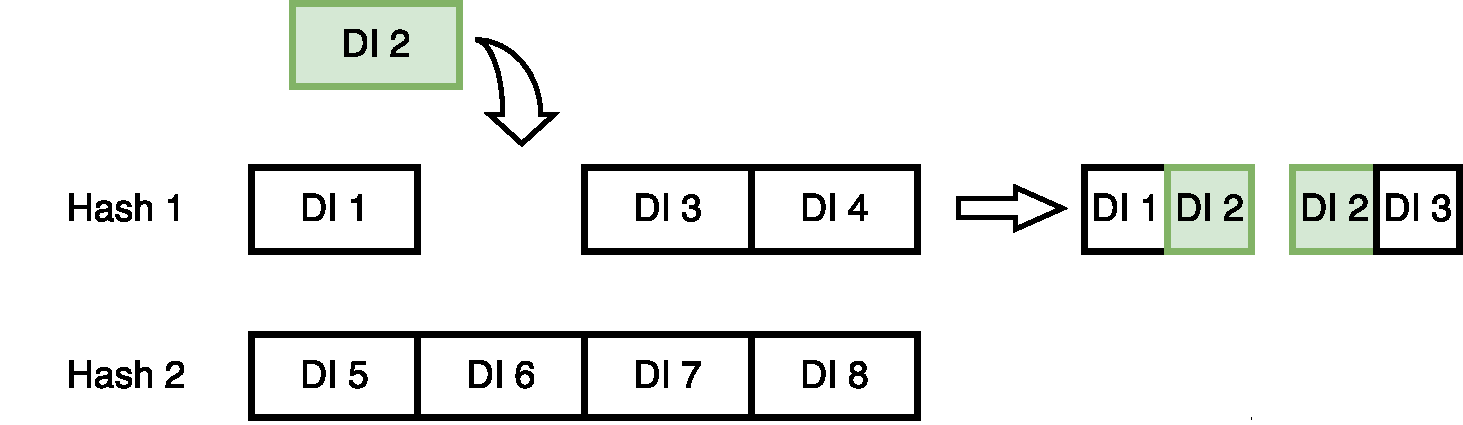
\includegraphics[width=0.48\textwidth]{pics/grouping-replaying}
  \caption{Replay in grouping}
  \label {grouping-replaying-figure}
\end{figure}

\subsubsection{Invalidation}
Replay can generate incorrect tuples, i.e. multiple tuples with the same last item. Therefore, only one tuple from such set is correct. To find out which tuples are incorrect we introduce the invalidation relation between two data items. Therefore, if new item {\it B} invalidates item {\it A}, item {\it B} can replace item {\it A}.

The data item {\it A} is said to be invalidated by the data item {\it B} if:
\begin{enumerate}
\item They have the same global time
\item The trace of {\it A} is lexicographically less than the trace of {\it B}
\item The first difference is in logical time
\end{enumerate}
If the first difference is in child id, e.g. they were generated by broadcast operation, there is no invalidation relation between them. Hence, the invalidation relation is a partial order. Notably, the invalidation relation cannot be lost, when item is go through other operations, because the trace of local times is append-only.

\subsubsection{Invalidation in grouping}
As it was mentioned above, grouping can generate incorrect tuples. Because of the cycles, such tuples can get back in grouping. Therefore, there is a need to remove them from the buckets, because they can lead to the unbounded number of invalid tuples in stream. Such behavior is implemented by removing items from bucket, if the item which invalidates them is arrived. Additionally, in order to generate all correct tuples, invalidation should trigger replay. 

The example of invalidation in grouping is shown on the figure~\ref{grouping-invalidation-figure}. In this example the green item invalidates red item. The window of grouping is 2.

\begin{figure}[htbp]
  \centering
  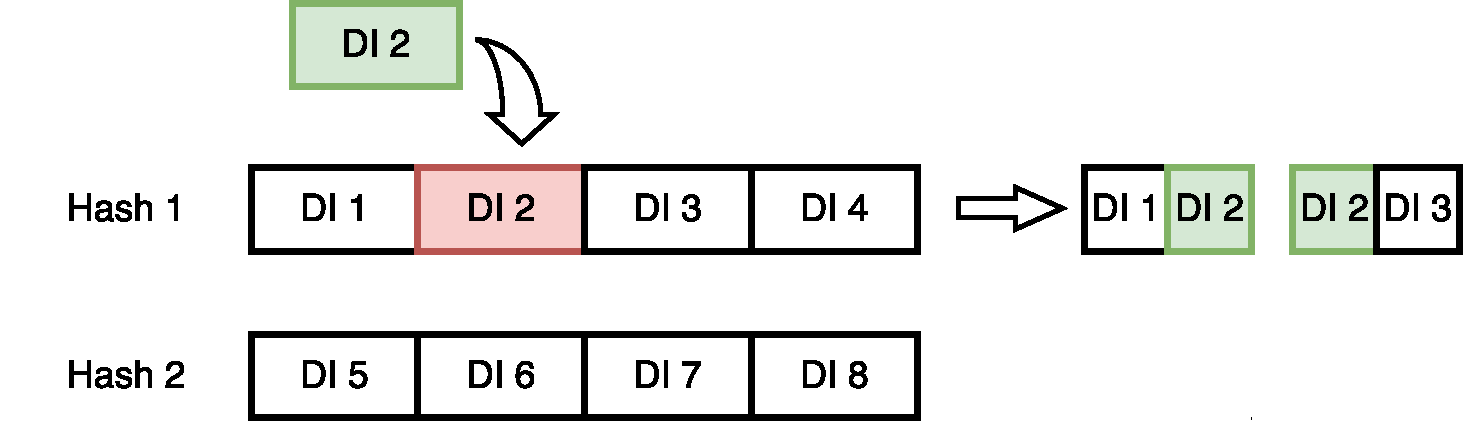
\includegraphics[width=0.48\textwidth]{pics/grouping-invalidation}
  \caption{Invalidation in grouping}
  \label {grouping-invalidation-figure}
\end{figure}

\subsection{Physical deployment and partitioning}

Each computational unit in our distributed runtime is assigned by integer interval. Intervals are not intersected and cover the range of 32-bit signed integer. Moreover, each unit contains complete logical graph.

As it was mentioned in the previous section, logical graph does not provide information about physical deployment. Physical graph extends logical one by assigning hash function to each input of each operation. This hash function is applied to the payload of data items and determines partitioning. More precisely, the value of hash function is computed before next operation and corresponding data item is sent to the unit which is responsible for the computed value. Therefore, load balancing explicitly depends on the hash functions of the operations. Optimal balancing requires the knowledge of payload distribution. Hence, the hash functions are assigned by business logic.

Notably, the hash function within grouping should be the same as partitioning hash function for grouping, because it guarantees that the result does not depend on the physical graph deployment. Other operations always do not depend on the physical graph, so they do not have this restriction.

Figure~\ref{logical-graph-figure} shows the example workflow of logical graph. Possible partitioning of this logical graph on two nodes is shown on the figure~\ref{physical-graph-figure}.

\begin{figure}[htbp]
  \centering
  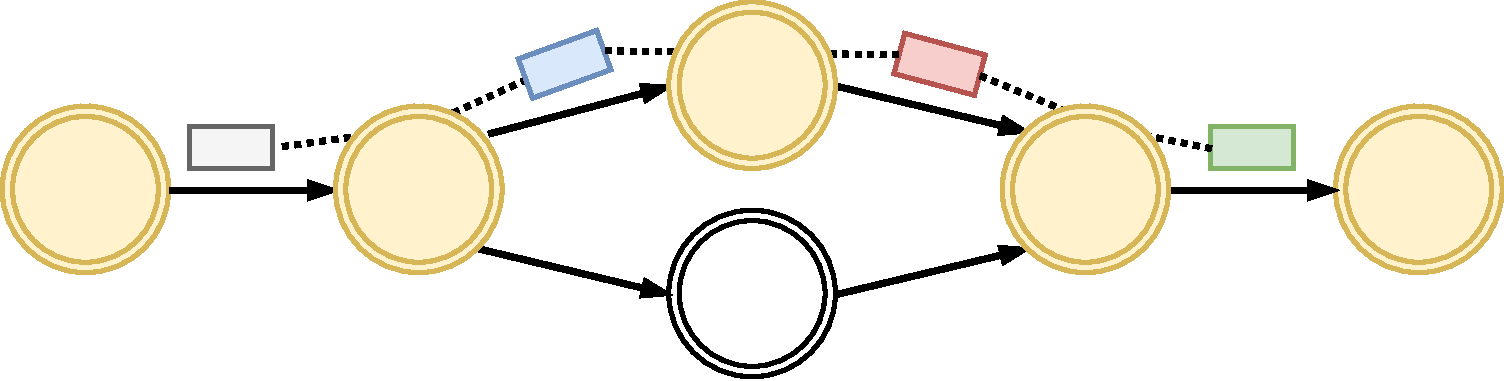
\includegraphics[width=0.48\textwidth]{pics/logical-graph}
  \caption{Logical graph workflow}
  \label {logical-graph-figure}
\end{figure}

\begin{figure}[htbp]
  \centering
  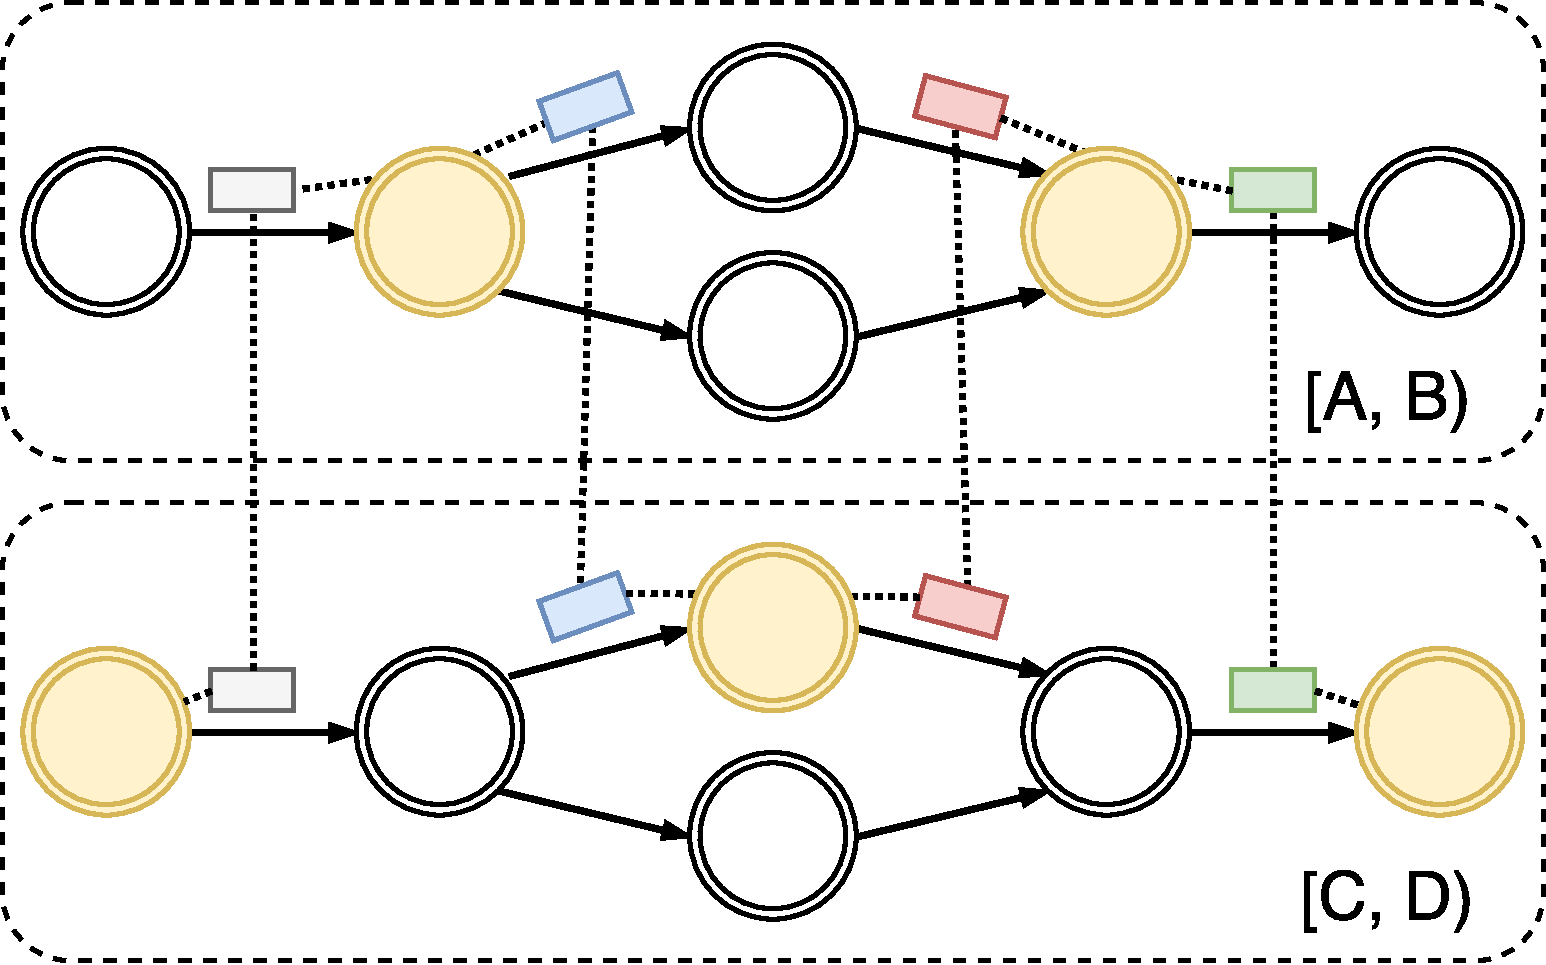
\includegraphics[width=0.48\textwidth]{pics/physical-graph}
  \caption{Possible partitioning of the logical graph}
  \label {physical-graph-figure}
\end{figure}

\subsection{System barriers}

\subsubsection{Front}
Front plays the role of data source. We assume that link between client's data and front is reliable and stable. The failure of this link is considered as the failure of client.

When data payloads are arrived at front, meta-information is assigned to them. As soon as the data obtains its meta-information, it is supposed that the system is responsible for this data. 

Each front is connected to corresponding operation. Similarly to the common physical graph vertex, data is sent to the appropriate node according to the value of hash function. Figure~\ref{front-figure} shows the example of interaction between client, front, and the other graph components.

\begin{figure}[htbp]
  \centering
  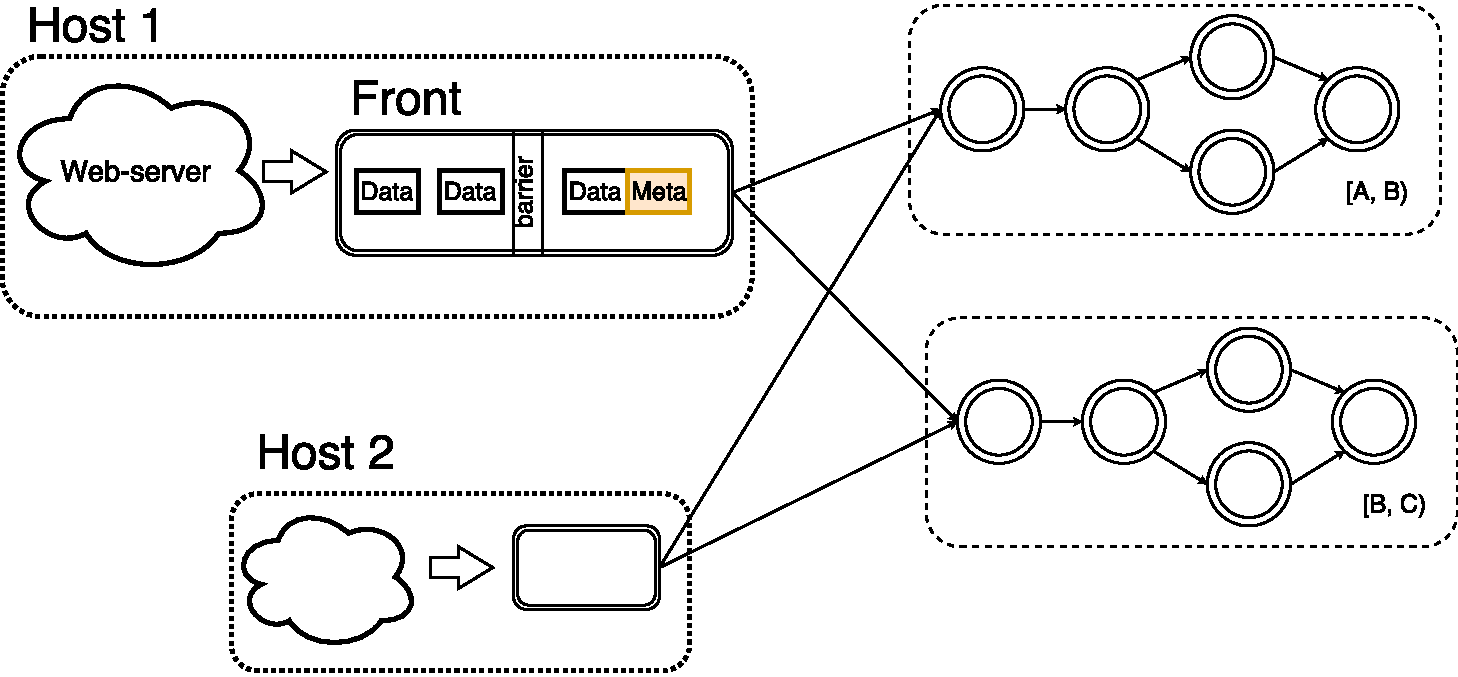
\includegraphics[width=0.48\textwidth]{pics/front}
  \caption{Example of fronts}
  \label {front-figure}
\end{figure}

\subsubsection{Sink}
Sink is the node which outputs items from the graph. It contains a buffer for data items. The items from buffer are released at some points in time. As it was mentioned above, grouping operation can generate invalid items. Consequently, there is a need to remove them from buffer before they get out from the system.  

However, there are two main difficulties. Firstly, sinks are the parts of the physical graph, so they are also partitioned by the business-logic hash function. Hence, item and corresponding invalidation item can arrive at distinct sinks. This issue can be solved by use of special partitioning for sinks by global time. Secondly, it is unclear when the items should be released from the buffer. To do it the system should ensure that there are no in-flight items which can invalidate items in buffer. The solution of this problem is detailed in the next section. 

Figure~\ref{invalidation-problems-figure} illustrates possible sink issues. Red items with labels 4 and 7 got out from the system, despite the fact that they should be invalidated by corresponding green items. 

\begin{figure}[htbp]
  \centering
  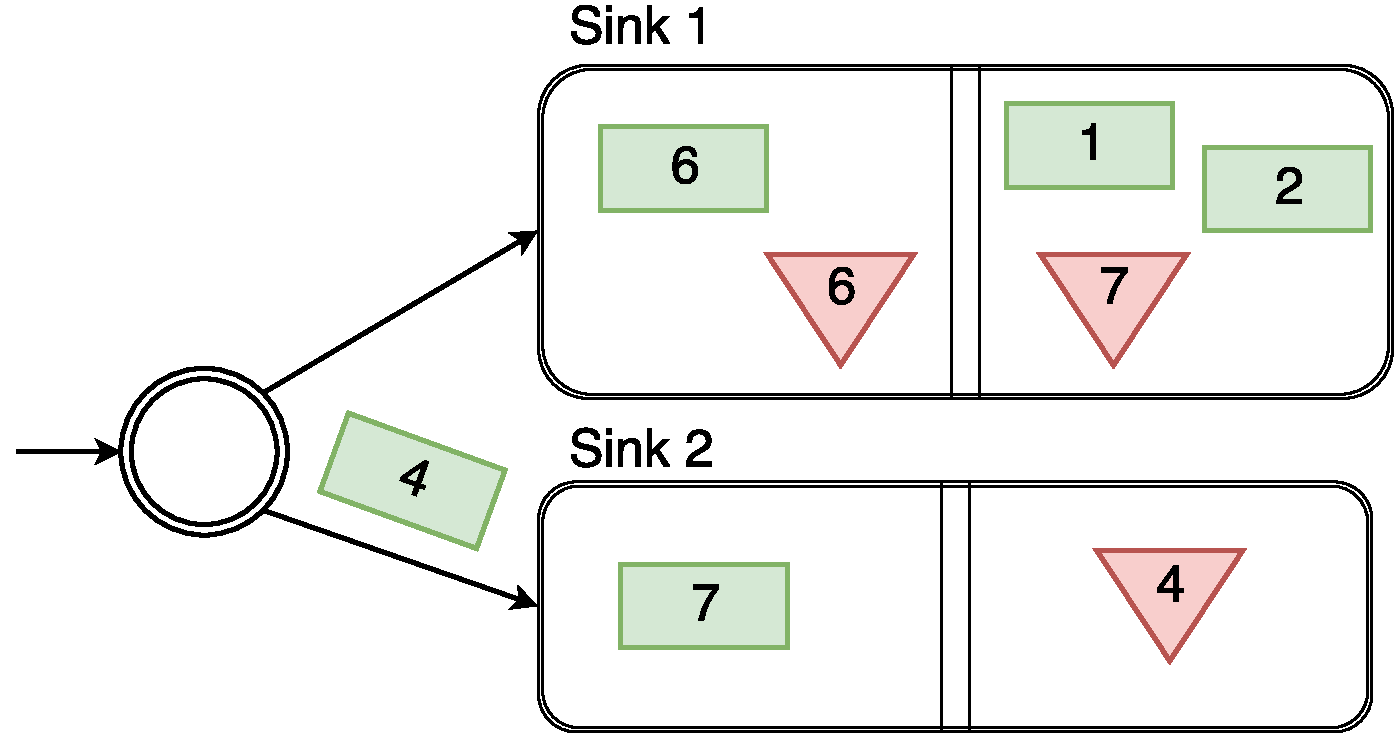
\includegraphics[width=0.48\textwidth]{pics/invalidation_problems}
  \caption{Possible sink issues}
  \label {invalidation-problems-figure}
\end{figure}

\subsection{Minimal time within stream}
In the previous subsection possible approach to output only correct items from sink was demonstrated. However, there is a need to ensure that there are no in-flight data items which can invalidate items in the sink buffer. In this subsection we offer sufficient condition that stream does not contain such items. Additionally, we describe how this condition is used in implementation.

\newtheorem{minimal-time-claim}{Claim}

\begin{minimal-time-claim}
Let {\it D} represent data item in sink buffer and let {\it GT} represent its global time. If the items with global time less than or equal to {\it GT} do not exist and cannot appear in the stream, then all items that invalidate {\it D} had already arrived at the sink buffer.
\end{minimal-time-claim}
\begin{proof}
Let {\it $D\prime$} invalidate {\it D}. According to the definition of invalidation relation, {\it $D\prime$} and {\it D} have the same global time {\it GT}, but different traces of local times. Let {\it LT} and {\it $LT\prime$} be the first distinct local times of {\it D} and {\it $D\prime$} respectively. Such difference could appear only as a result of grouping replay. Hence, {\it D} and {\it $D\prime$} are tuple items.

The global time of tuple item is inherited from the last item in the tuple, i.e. the last item in tuple {\it $D\prime$} has global time {\it GT}. Therefore, considering the properties of grouping operation, {\it $D\prime$} could be generated only if item with global time less than or equal to {\it GT} arrived at grouping. 

This implies that if stream does not contain items with global time less than or equal to {\it GT} and such items cannot appear, then all items which invalidate {\it D} had already arrived at sink buffer. 
\end{proof}

Regarding this claim, to output item from sink buffer we should ensure that:
\begin{enumerate}
    \item There are no items in stream with global time less than or equal to the global time of this item;
    \item Such items cannot be generated.
\end{enumerate}

To ensure that stream does not contain these items, we use module called {\it acker}. Its idea was proposed by Apache Storm \cite{apache:storm}. Acker tracks data item within the stream using a checksum hash. When item is sent or received by operation, its hash is XORed into the checksum. Therefore, if all items arrive at sink successfully, the checksum is zero. 

To find out the least global time of the items in stream, checksums are grouped by timestamps of global time into the structure called {\it ack table}. Hence, if the value of the specific timestamp in the ack table is zero, there are no items with corresponding global time into the stream. 

Notably, to ensure that no fronts would generate item with this timestamp, each front periodically sends to acker special message called {\it report}, which contains the least timestamp that can be assigned to data item by the front. The value in the ack table can become a zero only after corresponding report is arrived.  

\subsection{System architecture}

\subsubsection{FlameStream API}
To submit the graph, client should describe it in terms of predefined operations, specify fronts, sinks, and wrap them in a {\it tick}. Tick is a unit of graph deployment. It consists of an {\it tick start timestamp}, {\it duration}, {\it state dependencies}, {\it hash mappings} and the graph itself. Tick start timestamp and duration specify which data items belong to the tick, according to their global time. State dependencies represent the set of ticks, which the current tick depends on. Hash mapping shows the relation between hash ranges and computational units. 

Typically, ticks have duration of several seconds, and each tick depends on the state of the previous one. In the case of sudden load growth, subsequent ticks could be deployed with different hash mapping, splitting some hash ranges.

We suppose that the main client of FlameStream would be a system which builds graph based on declarative language. However, the performance of graph execution can be influenced by current load, the performance of operations, metrics, etc. Hence, frequent graph redeployment is a crucial goal for our system.

\subsubsection{Process model}
\begin{figure}[htbp]
  \centering
  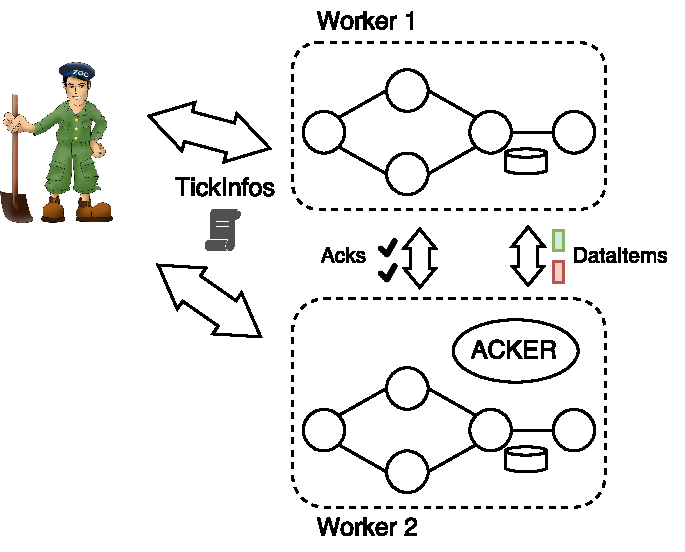
\includegraphics[width=0.48\textwidth]{pics/process-model}
  \caption{FlameStream process model}
  \label {process-model}
\end{figure}

Figure~\ref{process-model} shows the FlameStream process model. It is represented by a homogenous set of worker nodes and a Zookeeper~\cite{hunt2010zookeeper} cluster.  

The purpose of workers is to execute graph. Additionally, they manage corresponding part of the state. There is one worker for each hash range within tick. Acker is deployed to the randomly chosen worker. There is one acker per tick. 

Zookepeer is used for cluster configuration and coordination. Particularly, it stores cluster management information, mapping from IP to computation unit, workers and fronts locations, etc. Regarding coordination, it handles ticks and their statuses. Such extensive usage of Zookeeper mitigates the need for the dedicated master node.

To deploy a tick, client writes it to the Zookeeper. Workers are notified when the new tick appears. Initially, they wait for the relevant state if needed. After that, they set up a new graph.

\subsection{Fault-tolerance}
As it was mentioned above, our goal is to support exactly-once computation semantics. In failure-free case, it is trivial to provide such guarantees. In presence of process failures, system should be able to restore consistent state and replay lost items if any. FlameStream relies on reply property of a front. More precisely, it is expected that front is able to replay any number of events. For instance, front could be a file, database table, of message broker e.g. Apache Kafka~\cite{kreps2011kafka} or Amazon Kinesis~\cite{amazon:kinesis}. 

To prevent the whole stream replay from the beginning, consistent snapshots of operations' state are flushed to persistent storage. Additionally, information that is enough to restore read position of the fronts, e.g. offsets in file, is also spilled to storage. Further we call this information {\it determinants}.

On recovery, the state of operations is rollbacked to the most recent snapshot and fronts are restored with the corresponding determinants.

In the subsections, we describe how and when snapshots are taken.

\subsubsection{Commit protocol}
Commit protocol is a sequence of actions to take consistent snapshot. Snapshot is taken when the minimal time within the stream is equal to the end of the tick interval. It guarantees that there are no elements in stream that belong to the current tick. Commit protocol consists of the following steps: 

\begin{enumerate}
\item{Acker broadcasts message called {\it commit} to fronts and graph operations}
\item{As soon as operation receives commit, it flushes state that belongs to the tick. After that, it responses with message called {\it commit done}. Front responses with its determinant.}
\item{Once all responses are collected by acker, it records tick status in Zookeeper}
\end{enumerate}

\subsubsection{State properties}
The most important property of FlameStream's state is that its structure allows to start processing of the next tick without await of the previous one's commit. 

Grouping is the only operation in FlameStream that has state. Fortunately, it has a well-defined structure: buckets, that are ordered by meta information, one for each hash. Such bucket has interesting persistent properties. Particularly, the meta information of the elements from the next tick is strictly greater than meta-information of the previous one. Therefore, the bucket can be divided into two parts: prefix that relates to the first tick and suffix that relates to the second as shown on the figure~\ref{state-structure}. 

\begin{figure}[htbp]
  \centering
  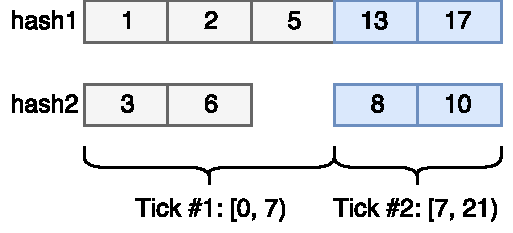
\includegraphics[width=0.48\textwidth]{pics/state-structure}
  \caption{State structure}
  \label {state-structure}
\end{figure}

When commit is initiated, grouping saves each bucket's prefix asynchronously to the next tick, because the next tick will not mess it up.

Non-blocking saving is possible, because in our model business logic state is a part of the stream as it was shown earlier. Hence, serialization, copy-on-write behavior, and immutability are already expressed in stateless operations.

\subsubsection{Guarantees}
At least once = on min time: State + replay + determinism

\subsubsection{Exactly once}
Exactly once = on min time: State + replay + determinism + idempotent sink

On commit: State + replay = Exactly once

